\subsection{风险监控失效}\label{sec:4}
风险管理需要不断监测公司所承担的风险并进行适当且及时的对冲,以确保公司承担它想承担的风险。彼时巴塞尔协议II主要强调资本这个单一维度,加之风险计量的复杂性和精确性也存在一定的缺陷。在混业经营的大背景下,部分大型银行凭借内部模型可用于监管资本计量的便利,推出了基于资产证券化、结构化融资以及信用衍生产品的各种金融创新,利用银行在风险计量模型和内部信息方面的不对称性进行监管资本套利,结果导致了系统性风险的大量累积。从这个角度上看,的确风险管理在当时存在缺陷。
\begin{figure}[H]
    \includegraphics[width=\linewidth]{img/basel.png}
    \caption{巴塞尔II对于系统性风险重视程度不足,且顺周期性过强}
\end{figure}

在巴塞尔II基础之上,各机构忽视了“房间里的大象”,这也是金融监管饱受诟病的。2006-07年各评级机构在竞争压力下失语,投行为了赚取更多佣金打包CDS为CDO,进一步吹大房贷市场的泡沫,最终引发了金融危机。例如ABX指数是CDS的平均加权平均值,代表AAA级证券化部分信用违约互换定价的AAA指数几乎没有变化,因此使用历史数据对AAA级证券化部分的风险进行合理评估时,应该是它们的风险很小。然而,这些证券的价值突然下跌,如图\ref{fig:abx}所示。如果次级证券的AAA评级部分的持有者选择使用ABX指数作为其所持证券价值的替代,他们会突然蒙受巨大损失。从这个角度看,08年金融危机风险管理的确存在失败。
\begin{figure}[H]
    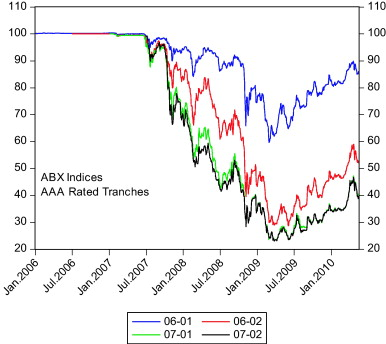
\includegraphics[width=\linewidth]{img/abx.jpg}
    \caption{ABX指数的波动}
    \label{fig:abx}
\end{figure}

风险监控失效的原因还有是监控风险的手段不一定能够做到准确及时。对于某些复杂衍生品,其风险属性可能会急剧变化。在同一天里,一个证券可能有一个利率风险敞口,如果利率上升,它就会有很大的收益,而在当天晚些时候,如果利率上升,它的风险敞口就会有很大的损失。对于这样的产品,每天调整的对冲可能最终造成巨大的损失,因为在一天开始时的最佳对冲可能最终加剧一天结束时的风险暴露。图\ref{fig:asia}是一个亚式期权的希腊值,随着时间变化希腊值的变化呈现阶梯式的跳跃,与欧式期权相对平缓的衰减完全不同。

\begin{figure}[H]
    \centering
    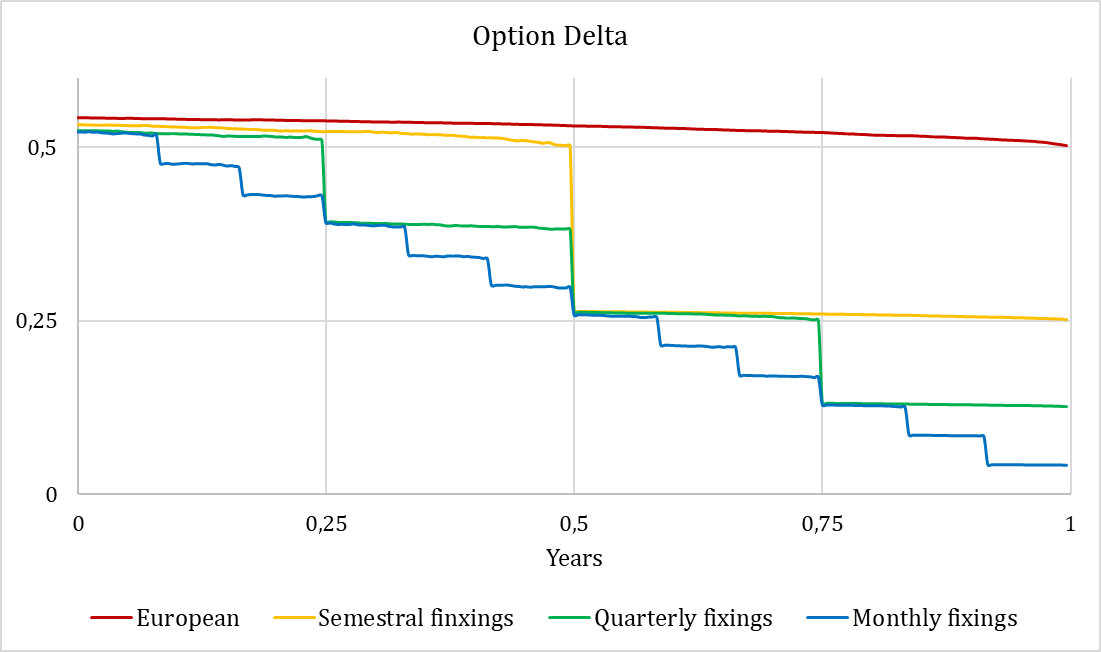
\includegraphics[width=\linewidth]{img/exo_delta.png}
    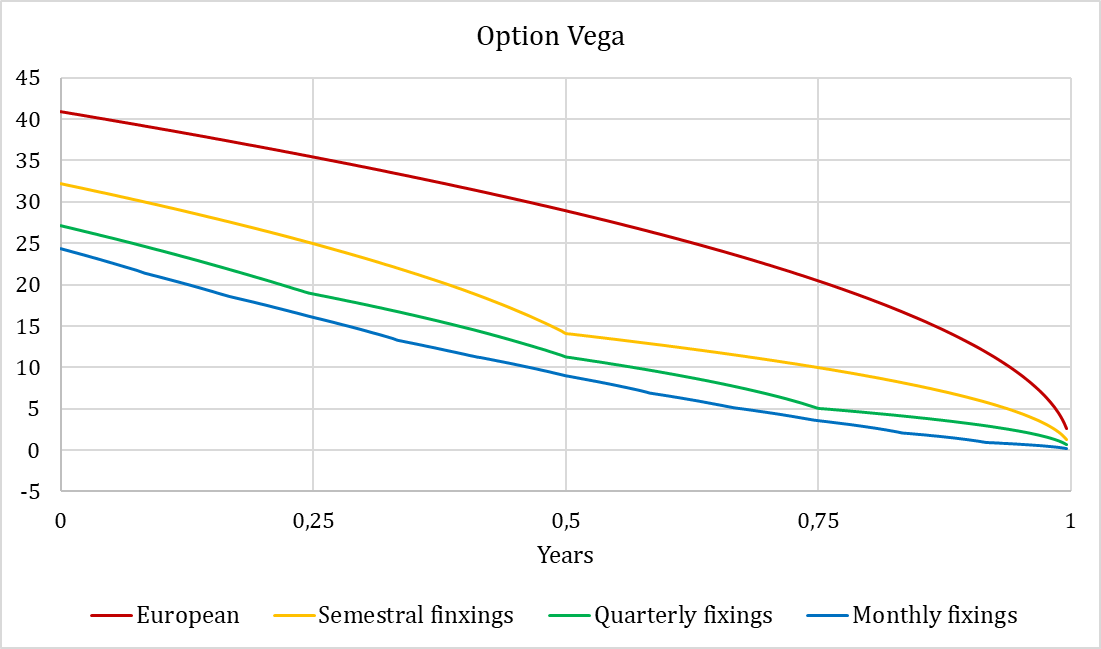
\includegraphics[width=\linewidth]{img/exo_vega.png}
    \caption{亚式期权的$greexotics$}
    \label{fig:asia}
\end{figure}

\subsection{风险管理措施失效}\label{sec:5}

风险管理的一个重要组成部分是确定可能的解决方案。如果一个公司可以在短时间内降低风险敞口,那么其潜在损失尚可控制。但当市场上大量公司卖出时,流动性可能会被抽干,导致许多在平时可以使用的风险管理方案就无法再使用。如图\ref{fig:libor}所示,雷曼破产使各金融机构加紧与交易对手清算,市场流动性大幅降低。
\begin{figure}[H]
    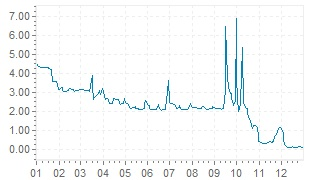
\includegraphics[width=\linewidth]{img/libor2008.jpg}
    \caption{2008年美元LIBOR报价}
    \label{fig:libor}
\end{figure}

按公允价值计量使大型组织更难估计风险和进行适当的对冲。对于大型组织来说,他们由于庞大的自身体量,参与到价格形成过程中时对价格影响非常大,使得他们做卖出决策时损失进一步放大。而随着按公允价值计量的损失被发现,其他机构也开始连锁调整,并进一步影响可能的交易价格。这一点在近两年的Bill Huang爆仓、英国养老金爆仓等案中尤为突出。
\begin{figure}[H]
    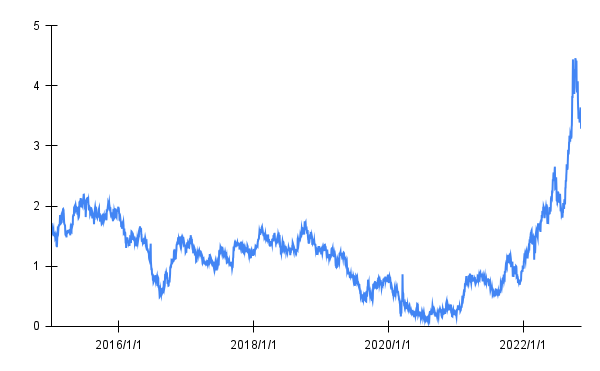
\includegraphics[width=\linewidth]{img/british_bond.png}
    \caption{英国养老金平仓补交保证金导致进一步踩踏}
\end{figure}

\subsection{未使用适当的风险衡量标准}\label{sec:6}
彼时及至今日,金融机构中广泛使用的风险度量标准是每日的VaR,短期VaR的衡量标准可能很低,公司可能看起来在这方面做得非常好,然而它也可能失败。VaR的缺陷包括:
\begin{enumerate}
    \item VaR不满足一致性
    \item 交易员可以在不违反VaR额度的前提下,构造一个较大风险的交易组合
    \item 资产价值不一定满足正态分布
    \item 交易组合价值变化在每天之间不一定相互独立
    \item 资产不一定可以被快速卖出或对冲(即\nameref{sec:5})
\end{enumerate}

解决方法是金融机构应该一方面考虑更长期的VaR,另一方面也要进行情景分析补充。

\section{更全面的风险管理如何规避危机:币安vs FTX}

前面我们的分析可以看出,金融危机暴露了彼时风险管理许多问题,但是并不意味着风险管理存在问题就一定会导致金融危机。我们也无法后验地判断通过全面风险管理成功规避了一次金融危机:阻止危机于危机形成之前也正是风险管理的价值所在。于此同时如今加密货币风起云涌,$7\times 24$小时的加密货币交易也包含了数次金融周期。我们试以两大中心化交易所FTX的倒下与币安的存活,来观察更全面的风险管理是如何发挥作用的。

\subsection{背景:LUNA归零、美联储加息}

在美联储加息大背景下,全球热钱迅速减少,以比特币、以太坊为代表的加密货币交易量趋于平缓,其价格也开启了跌跌不休的模式。

\begin{figure}[H]
    \begin{minipage}[t]{0.48\linewidth}
        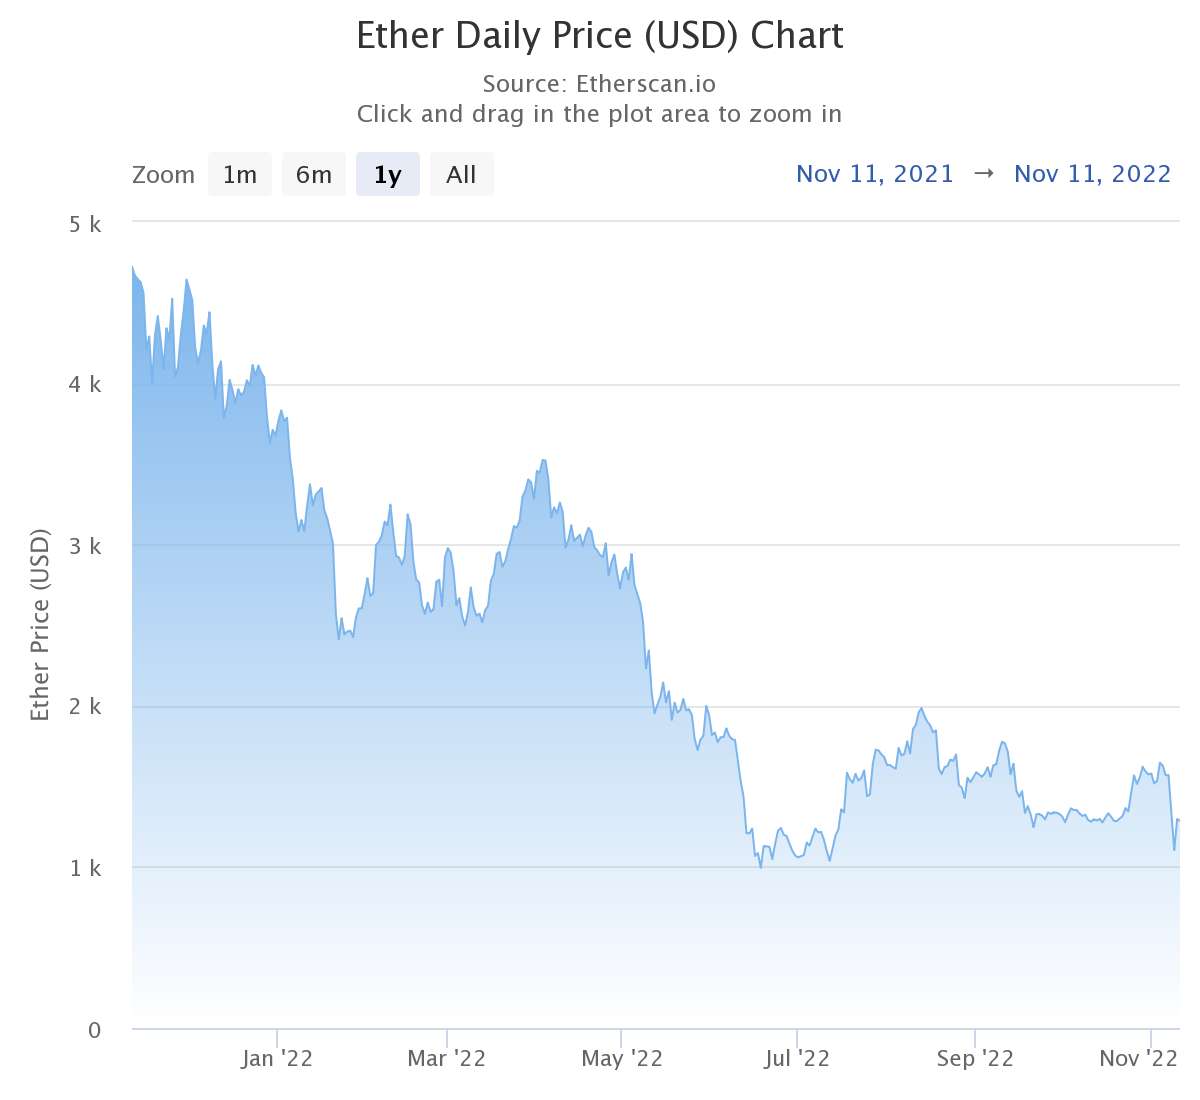
\includegraphics[width=\linewidth]{img/ether-daily-price-usd-ch.png}
        \caption{以太坊价格大幅回调}
    \end{minipage}
    \begin{minipage}[t]{0.48\linewidth}
        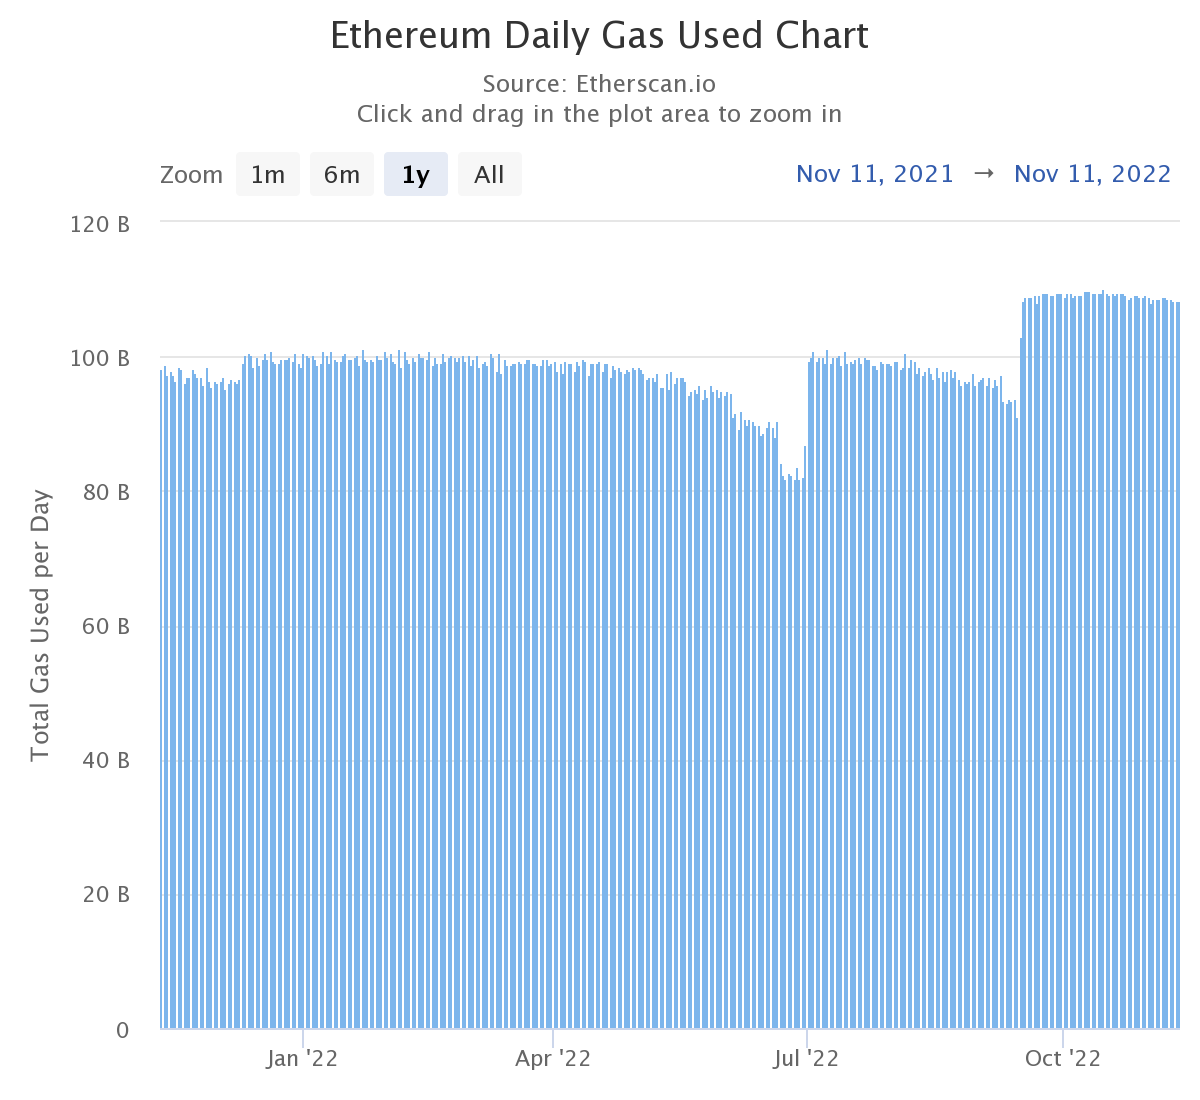
\includegraphics[width=\linewidth]{img/ethereum-daily-gas-used.png}
        \caption{以太坊交易量增长放缓}
    \end{minipage}
\end{figure}

LUNA是今年来暴雷的加密货币之一。浮动价格的LUNA的应用是发行币值1美元的UST,每发行1美元的UST即销毁价值1美元的LUNA,反之亦然。而为了吸引人前来铸造UST完成左脚踩右脚的上升循环,LUNA官方推出了20\%定期收益的UST存款业务,吸引用户使用UST,70\%的UST存在该合约中。LUNA的价格也水涨船高,市值最高达410亿美元。但随着加息周期的到来,大量资金流出,销毁UST铸造LUNA,导致LUNA价格暴跌。
\begin{figure}
    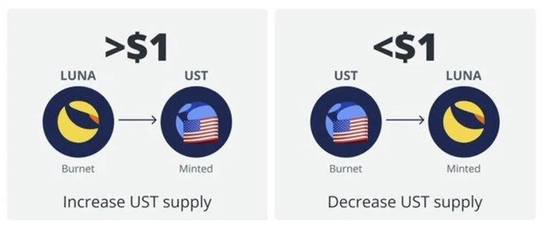
\includegraphics[width=\linewidth]{img/ust.jpeg}
    \caption{LUNA/UST的关系}
\end{figure}
\begin{figure}
    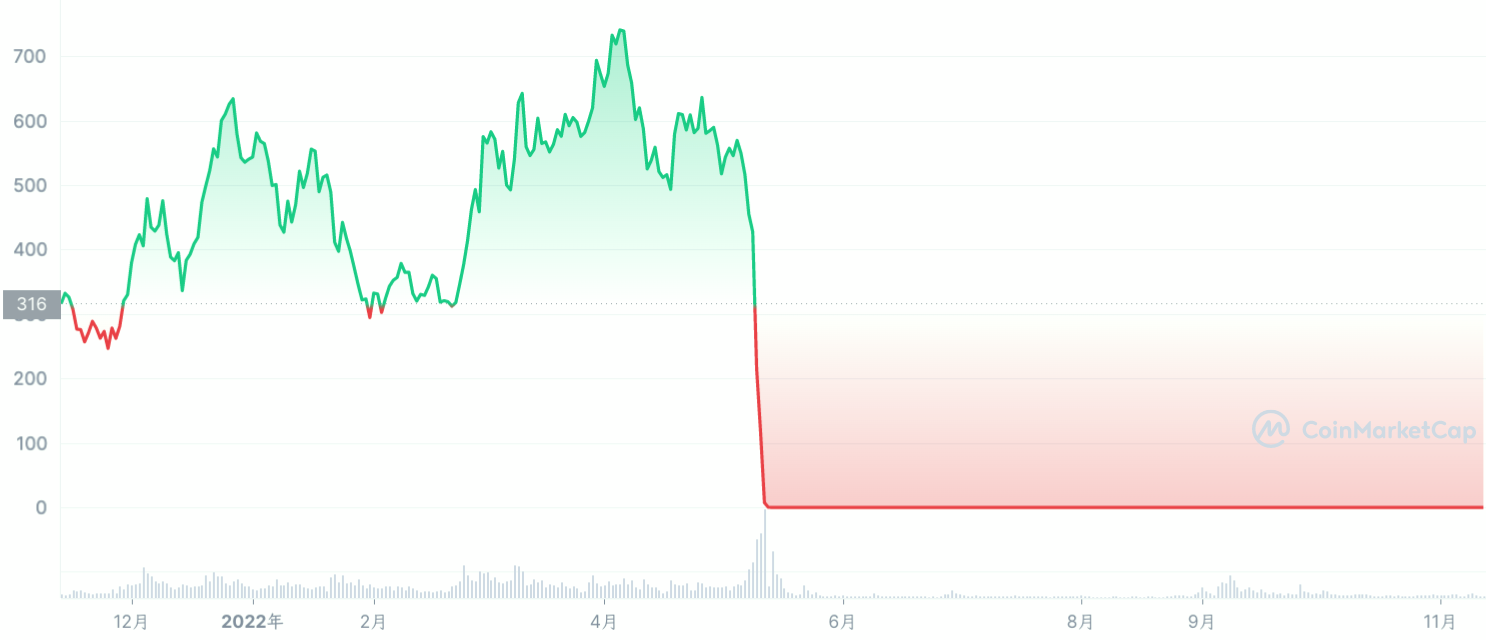
\includegraphics[width=\linewidth]{img/luna.png}
    \caption{LUNA从120美元跌至0.00014美元}
\end{figure}

LUNA的暴跌带动加密货币全线大跌,压垮了多家风投机构,包括Voyager、Celsius、3AC等数家AUM数十亿美元的机构。加密货币两大交易所币安和FTX均尝试购买这些机构的剩余资产包,最终FTX在竞价中胜出。
\subsection{FTX的坠落:风险管理失败的例子}
FTX由Sam Bankman-Fried(SBF)创立,在量化对冲基金中的经历使SBF信奉“从长期来看,风险爱好者和风险规避者都会输给风险中立者”。FTX发行了FTT作为FTX的“股票”,以衍生品交易见长。在SBF高调成为美国民主党第二大捐助者后不久,FTT暴跌、FTX不得不宣布破产。
\begin{figure}
    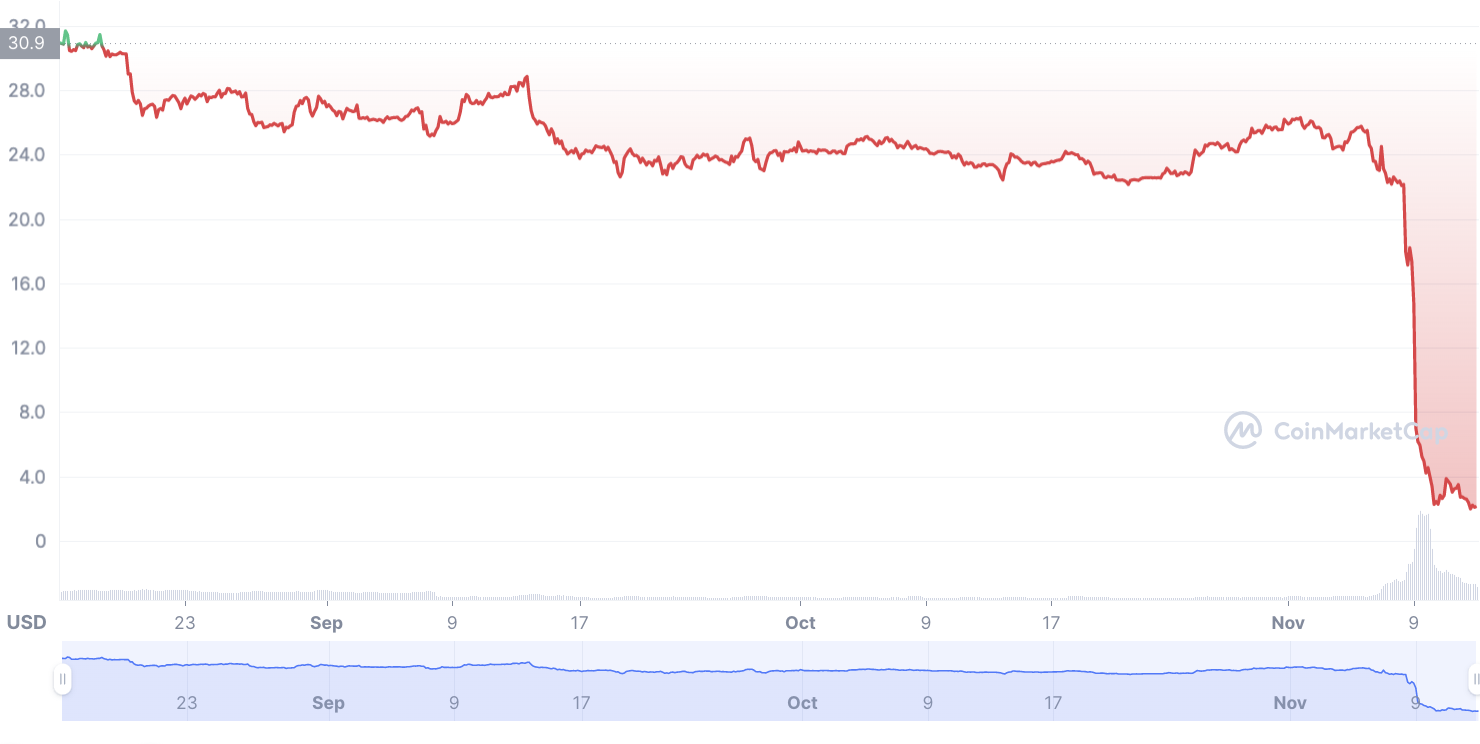
\includegraphics[width=\linewidth]{img/ftt.png}
    \caption{FTT暴跌}
\end{figure}

SBF的另一家公司Alameda Research为FTX上的做市商,提供流动性并赚取价差。我们可以看出SBF犯了上一章中指出的许多错误,令FTX从全球交易所日交易量排名第4位跌入破产深渊,Alameda其资产负债表如表\ref{fig:bs}所示
\begin{figure}[H]
    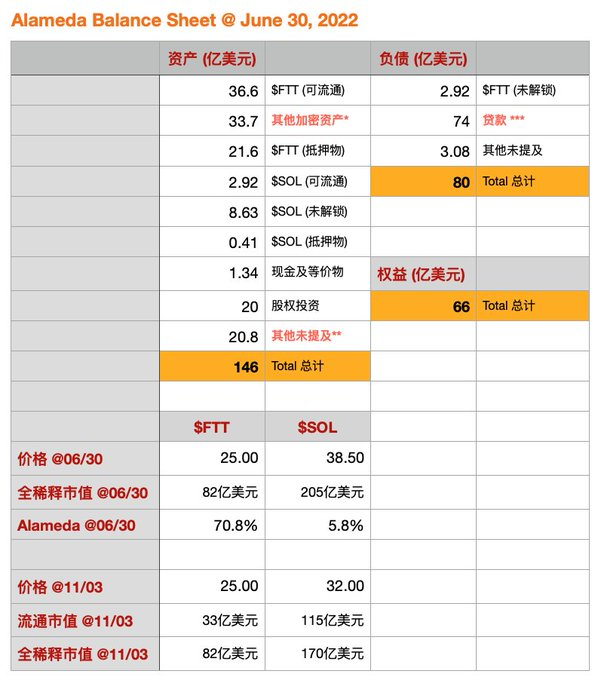
\includegraphics[width=\linewidth]{img/alameda_bs.jpeg}
    \caption{Coindesk曝光的Alameda资产负债表}\label{fig:bs}
\end{figure}

逐条分析SBF的风险管理措施,我们可以发现:
\begin{enumerate}
    \item \textbf{\nameref{sec:1}}:FTX和Alameda大肆收购了Voyager、Celsius等资产包,这些有毒资产消耗了大量的现金同时,也提高了FTX的杠杆率。而为了在加密寒冬中维持正常扩张、挑战币安地位,SBF暗中挪用了用户部分资金,迄今累计挪用接近100亿美元。
    \item \textbf{\nameref{sec:2}}:SBF和Alameda以量化套利起家,其资金来源为在FTX套利过程中的资金沉淀,并以此进行短贷长投增厚收益。这种行为没有考虑到挤兑风险:在过去加密市场上行时,更多的用户进入市场使得这种行为可持续;而当加密寒冬到来时,用户提款可能会形成挤兑压倒FTX。
    \item \textbf{\nameref{sec:3}}:Alameda资产负债表被曝光后,Alameda CEO曾表示愿以22美元的价格回购FTT,但面临5亿美元的缺口FTX管理层集体失联,导致市场信心进一步下挫,恐慌情绪蔓延。
    \item \textbf{\nameref{sec:4}}:Alameda资产负债表两侧对于加密货币价格敏感程度差异巨大,没有对冲加密货币波动。Alameda利用FTT作为FTX的抵押品,从FTX借入其他资产,例如美元支持的稳定币。而在资产端为加密货币纯多头,在FTT价格波动较低时尚可平衡,而当整体加密货币向不利方向异常波动时容易资不抵债。
    \item \textbf{\nameref{sec:5}}:Alameda资产中大部分为FTT,FTT完全稀释市值为88.84 亿美元,而FTX就持有超过50亿美元,考虑到流动性,若短时间大量抛售将难以维持最初估值。
    \item \textbf{\nameref{sec:6}}:SBF信奉“风险中性者在长期期望上胜过风险爱好者和风险规避者”,FTX的风险衡量标准仅仅是“资产>负债”,在危机爆发初期SBF称其有能力支付用户存款。可当资产快速贬值时,该风险衡量标准缺陷暴露无疑,最终走向破产。
\end{enumerate}

\subsection{币安何以坚挺:风险管理如何规避危机}
与FTX类似,币安作为全球最大的加密货币交易所也提供了不少衍生品合约,但币安却在加密货币暴雷潮中幸免于难。

\section{结论}

我们倾向于认为金融危机是不全面的风险管理的失败。金融危机产生于不全面的风险管理问题的集中爆发,例如对信贷市场的错误估计、衍生品的监管、金融机构的监管套利、流动性风险的长期忽视等等。风险管理也在金融危机中学习教训进一步补完,在经过金融危机历练后风险管理也在进一步地改善,如更为完善的监管体系、对流动性风险由定性转化为定量要求等,风险管理仍是有价值有意义的。
